\documentclass[12pt,a4paper]{report}
\usepackage{graphicx}
\usepackage{ltablex}
\usepackage{adjustbox, array, hhline}
\usepackage{makecell}
\renewcommand\theadfont{\normalfont\bfseries}
\setcellgapes{4pt}
\usepackage{geometry}
 \geometry{
 a4paper,
 top=30mm,
 }
 \usepackage{makeidx}
\makeindex

\usepackage{graphicx}
\usepackage{longtable}
\usepackage{array,multirow}
\usepackage{sectsty}
\usepackage{caption} 
\usepackage{color}
\usepackage{tabularx}
\usepackage{amsmath}
\usepackage{ltablex}
\usepackage{adjustbox, array, hhline}
\usepackage{makecell}
\usepackage{cite}
\usepackage[nottoc]{tocbibind}
\usepackage{enumitem}
\usepackage{booktabs}
\usepackage{threeparttablex}
\usepackage{ragged2e}
\usepackage{amsfonts}
\usepackage{setspace}
\usepackage{fancyhdr}
\renewcommand\theadfont{\normalfont\bfseries}
\setcellgapes{4pt}
\graphicspath{{F:/photos/}}
\usepackage{wrapfig}
	

\captionsetup[table]{skip=10pt}
\usepackage{hyperref}



\begin{document}
\begin{titlepage}
	\centering
      	{\large \textbf{A secured mobile app for maintaining
Personal diary}\par}
      	\vspace{0.5cm}
	A project submitted to 
	
	\vspace{1cm}
	\graphicspath{ {F:/0/} }

	
	{\textbf{MIT SOE}\par}
	\vspace{0.5cm}
	in fulfilment of the requirements for the degree of\par
	\vspace{0.5cm}
	{\Large \textbf{B.Tech}\par}
	\vspace{0.5cm}
	in\par
	\textbf{Information Technology \& Engineering}\par
	\textbf{Under the Faculty of Engineering \& Technology}\par
	\vspace{2cm}
	 Submitted by\\
	{\Large \textbf{Prachi  2*****}\par}
	
	\vspace{1cm}
		
	\vspace{1.1cm}
	 Under the Guidance of\\
	{\Large \textbf{Prof.XXX XXXX}\par}
	
	\vspace{1.1cm}
	
	
\includegraphics{mit.png}
		\vspace{1cm}   
	
	Place of Research Work\\
	\vspace{0.2cm}
	\textbf{DEPARTMENT OF Information Technology \& ENGINEERING}\par
	\textbf{MITSOE \\
	MITADT}

	\vspace{0.3cm}
	[JANUARY 2020]
	% Bottom of the page
	
\end{titlepage}
      	 





\captionsetup[table]{skip=10pt}




\pagenumbering{gobble} 
\chapterfont{\centering}
\chapter *{ACKNOWLEDGEMENT}
\large 
Getting a project done reflects the proverbial saying “Success is a marathon and not a sprint”. Dedication and perseverence when supported by inspiration and guidance leads to success. We’re highly indebted to Prof. XXXXXX XXXXXX for their guidance and constant supervision as well as for providing necessary information regarding the project & also for their support in completing the Mini Project work. In true sense it was privilege for us to have him as our guide and we felt highly honored working under him.
\par
Prof.(Dr.) XXXXX XXXXXXXXX, Head, Dept. of Information Technology, has been a constant source of inspiration to us. Both are responsible for giving us the confidence and courage throughout execution. 
\par
We do not have words to express our sincere thanks to Prof. (Dr.) XXXXXXX XXXXXX, Principal-MIT School of Engineering for their constant support and encouragement throughout the Mini Project work.
\par
We also acknowledge the help of family, friends and all those who have encouraged and helped us directly or indirectly with our work but whose contribution we may have failed to mention inadvertently. 

\vspace{5cm}



\begin{tabular}{p{1cm}>{\raggedleft\arraybackslash}p{11.5cm}}
& Prachi (2XXXXXX) \\

 & TY IT \\
 \end{tabular}

\tableofcontents



\chapter*{\textbf{ABSTRACT}}

\Large	
\addcontentsline{toc}{chapter}{\textbf{Abstract}}
Applications has proved its importance in many aspects of human life and they are becoming one of the reliable sources of getting information from the internet through application specific task. We all must have decide to write diary at least once? What is new in it we may take our pen and book out and can write the dairy but is it maintaining consistency? No.This application takes care that you must be consistent in writing you diary by scheduling and maintaining the work related information.It means this application will allow you to keep track on your study field and also for official use.
 

\hspace{1cm}\listoffigures
\clearpage
\listoftables
\clearpage
\pagenumbering{arabic}
\pagestyle{fancy}
\fancyhf{}
\fancyhead[R]{\tiny \leftmark} 
\cfoot[\hline ]{\thepage}
\renewcommand{\headrulewidth}{0pt}
\renewcommand{\footrulewidth}{0pt}




\chapterfont{}
\setcounter{secnumdepth}{4}
\chapter {INTRODUCTION}
The first thing while writing a personal diary everyone is concerned with is it's privacy. Even when kept carefully, our diary can be read by anyone who happens upon them. This Digital Personal Diary application will help your personal details and your regular diary writing in safe hand as it is safe with google authentication system, so you can rest easy knowing that all your entries are secure in the Digital Diary.
\par 
Students can update diary anytime anywhere and can also have multiple diaries. Each student diary is secured with password and can get contents of diary with respect to date.

\section{Problem Statement: }
\par A secured mobile app for maintaining Personal Diary.
\par Previously, the system holds only to manage the note of the dairy. We  were using separate applications for reminder of tasks, the task of managing daily task or future task. So we have developed this MyDairy application to overcome the existing problem with the modules like MyDairy, My Tasks, Holidays, Timetable and Feedback in one application. 

\section{Ojectives: }
\begin{enumerate}[label=\roman*.]
\item To provide a virtual experience of digital dairy.
\item To provide latest information about the time table, holidays and upcoming events 
\item To design an application which will have administrator account who will manage the holiday lists, timetable and feedback. 
\item To give platform to the students to manage their tasks and create their own personal space in the form of notes. 
\end{enumerate}

\section{Features: }
\begin{enumerate}[label=\roman*.]
\item Google Authentication for password: Through this service one can access their account in DigiPersonal Diary through one step security by their own email id.
\item Daily diary writing system: One can freely record personal daily experiences.
\item Event notification and updates: This software provides notificationary feature which help in the form of a remainder.
\item Display holiday list: A collection of all holiday list throughout the academic year.
\item Feedback module: A satisfactory way for the administration to know about the compiling of the application.
\item Time Table notification module: One more notificationary way to know the upcoming lectures in the form of remiander.
\end{enumerate}

\section{Organization of Report: }
In the chapter 1, we introduced the problem in the existing system and explained the proposed system along with problem statement, objectives and features. Chapter 2 provides project system design. Chapter 3 consists of the technology and system implementation results and analysis. Chapter 4 comprises of system application. In the chapter 5, conclusion and future scope is provided.




\chapterfont{}
\setcounter{secnumdepth}{4}
\chapter {SYSTEM DESIGN}
\section{Use Case Diagram}
Diagram:
\begin{figure}[h]
    \centering
    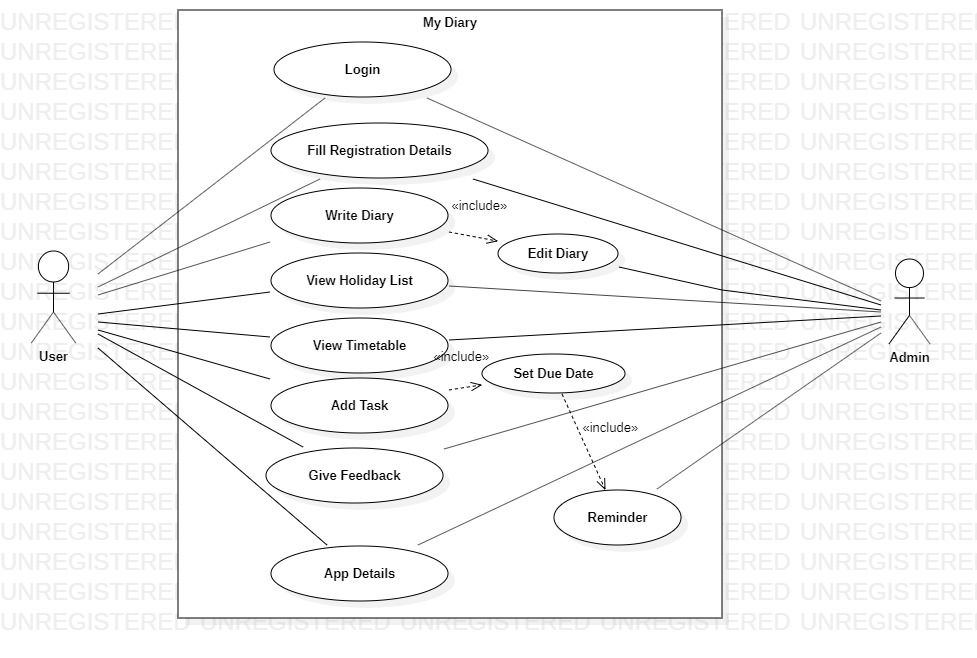
\includegraphics[width=12cm,height=10cm]{usecase.jpeg}
    \caption{Use Case Diagram}
    \label{fig:my_label}
\end{figure}
    

\section{Class Diagram}
Diagram:
\begin{figure}[h]
\centering
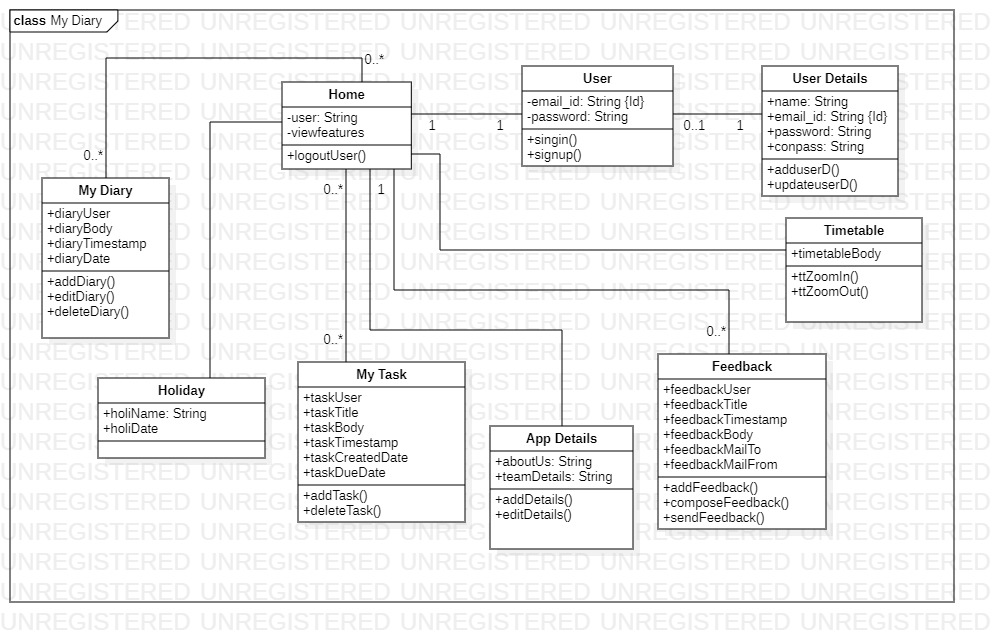
\includegraphics[width=.7\textwidth]{class.jpeg}
\caption{Class Diagram}
\label{fig:my_label}
\end{figure}


\section{Sequence Diagram}
Diagram:
\begin{figure}[h]
\centering
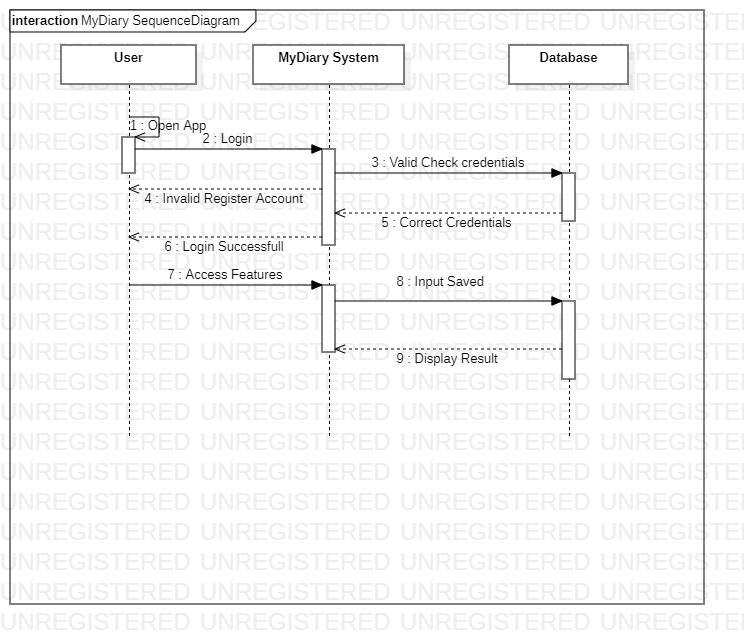
\includegraphics[width=.7\textwidth]{sequence.jpeg}
\caption{Sequence Diagram}
\label{fig:my_label}
\end{figure}
    
   
\section{Activity Diagram}
Diagram:
\begin{figure}[h]
    \centering
    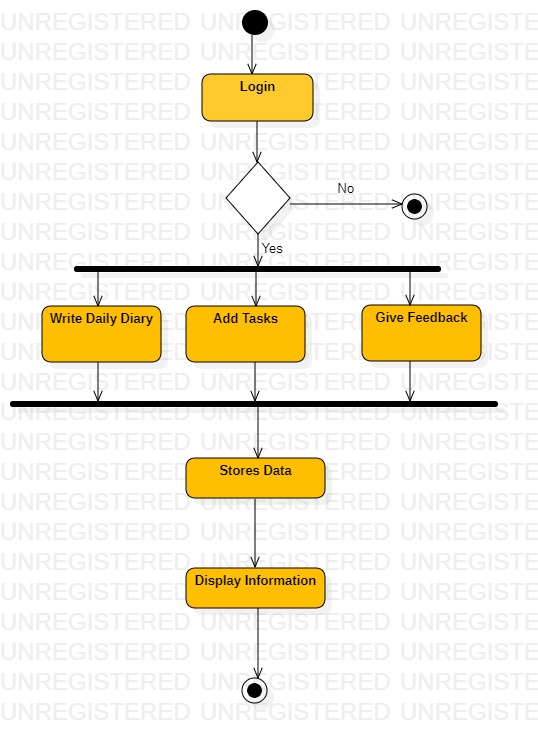
\includegraphics[width=10cm,height=8cm]{activity.jpeg}
    \caption{Activity Diagram}
    \label{fig:my_label}
\end{figure}

\begin{table}[ht]
\centering
    \caption{Test Case for Login usecase}
    \scalebox{1}{
    \begin{tabular}{|c|c|c|}
    \hline
    Test Cases  & Steps & Expected Result \\
    \hline
    \hline
    \hline
    A  & \multicolumn{2}{c|}{Login-Normal form} \\
    \cline{2-3}
    \hline
    \hline
    1 & Enter username & User can enter Username\\
    \hline
    2 & Enter password & User can enter Password\\
    \hline
    3 & Click on Signin & System gives User Signin\\
    \hline
    \hline
 
     B & \multicolumn{2}{c|}{Login-Invalid Username}\\
     \cline{2-3}
    \hline
    \hline
    1 & Repeat steps of 1,2,3 of Signin & \\
    \hline
    2 & Enter username & System displays Error message \\
    \hline
    \end{tabular}}
\end{table}

\newpage
\section{Database Design}
    \begin{table}[ht]
    \centering
    \caption{Notes}
    \scalebox{1}{
    \begin{tabular}{|c|c|c|}
    \hline
    Collections  & Feilds & Datatype \\
    \hline
    notes& date & timestamp\\
    \cline{2-3}
     & name & string\\
    \cline{2-3}
    & note & string\\
    \cline{2-3}
    & uid & string\\
     \hline
    \end{tabular}}
    \end{table}


\begin{table}[ht]
    \centering
    \caption{Tasks}
    \scalebox{1}{
    \begin{tabular}{|c|c|c|}
    \hline
    Collections  & Feilds & Datatype \\
    \hline
     tasks & createdOn & timestamp\\
    \cline{2-3}
     & dueOn & timestamp\\
    \cline{2-3}
    & name & string\\
    \cline{2-3}
    & note & string\\
    \cline{2-3}
    & title & string\\
    \cline{2-3}
    & uid & string\\
     \hline
    \end{tabular}}
    \end{table}


\begin{table}[ht]
    \centering
    \caption{Users}
    \scalebox{1}{
    \begin{tabular}{|c|c|c|}
    \hline
    Collections  & Feilds & Datatype \\
    \hline
     users & email & string\\
    \cline{2-3}
     & name & string\\
    \cline{2-3}
    & uuid & string\\
    \hline
    \end{tabular}}
    \end{table}
    
    


\chapterfont{}
\setcounter{secnumdepth}{4}
\chapter {SYSTEM IMPLEMENTATION}
\section{Technology}
\textbf{Platform:}Windows\\
\\
\textbf{Front End:}\\
React Native(Framework) : React Native renders native applications for both iOS and Android mobiles.React components wrap existing native code and interact with native APIs via React’s declarative UI paradigm and JavaScript.It has been designed to seamlessly work with Objective C and Java wherever required, which allows is to integrate React JS features into native code. \\\\
Expo : An open-source platform for making universal native apps with React. Expo runs on Android, iOS, and the web. Build service gives you app-store ready binaries and handles certificates, no need for you to touch Xcode or Android Studio.\\\\          
\textbf{Backend:}\\
Firebase(Database) : Firebase Authentication provides backend services, easy-to-use SDKs, and ready-made UI libraries to authenticate users to your app. It supports authentication using passwords, phone numbers, popular federated identity providers like Google, Facebook, TWitter, and more.\\\\
JavaScript : React Native combines the best parts of native development with React, a best-in-clas Javascript library for building user interfaces. React Native is a cross-platform mobile development on the other side uses Javascript as it coding language but it compiles its components in native code.

\section{Results and Analysis}

\begin{figure}[h]
\makebox[\textwidth]{%
    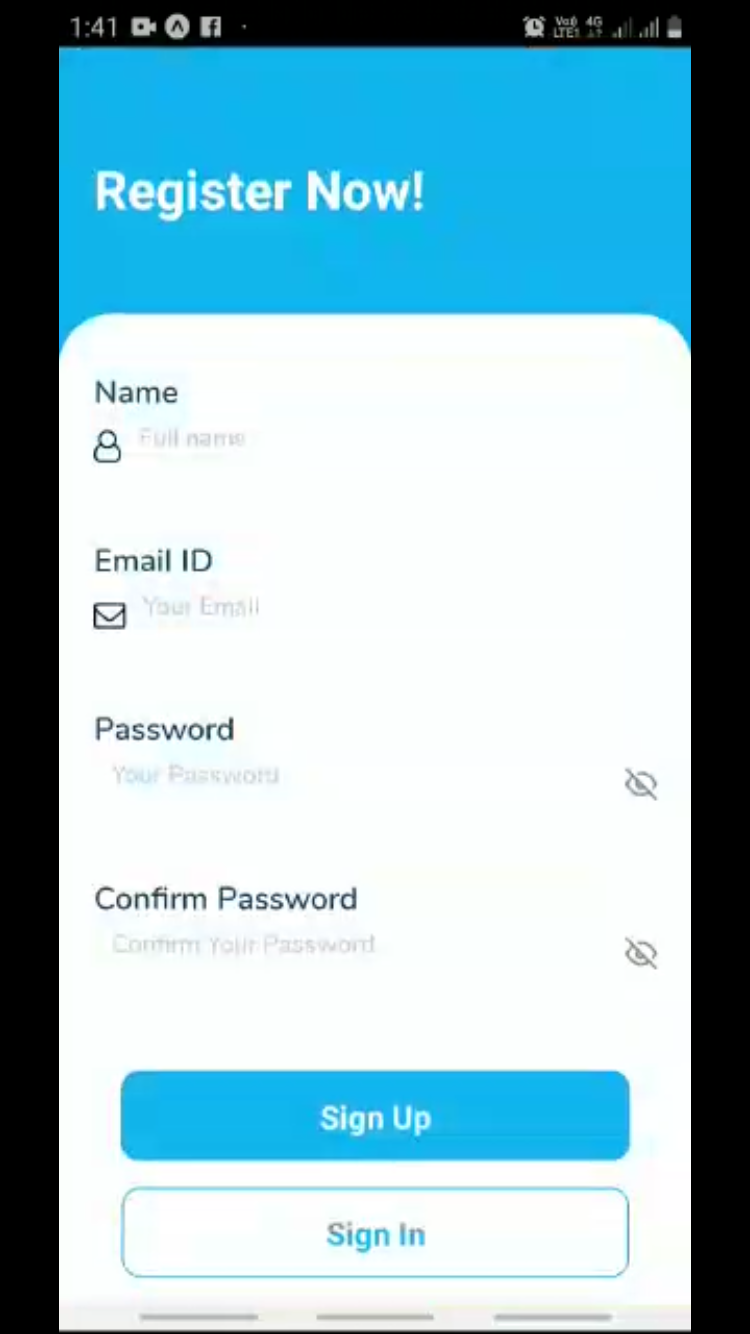
\includegraphics[width=0.49\textwidth]{register.PNG}%
    \hfill
    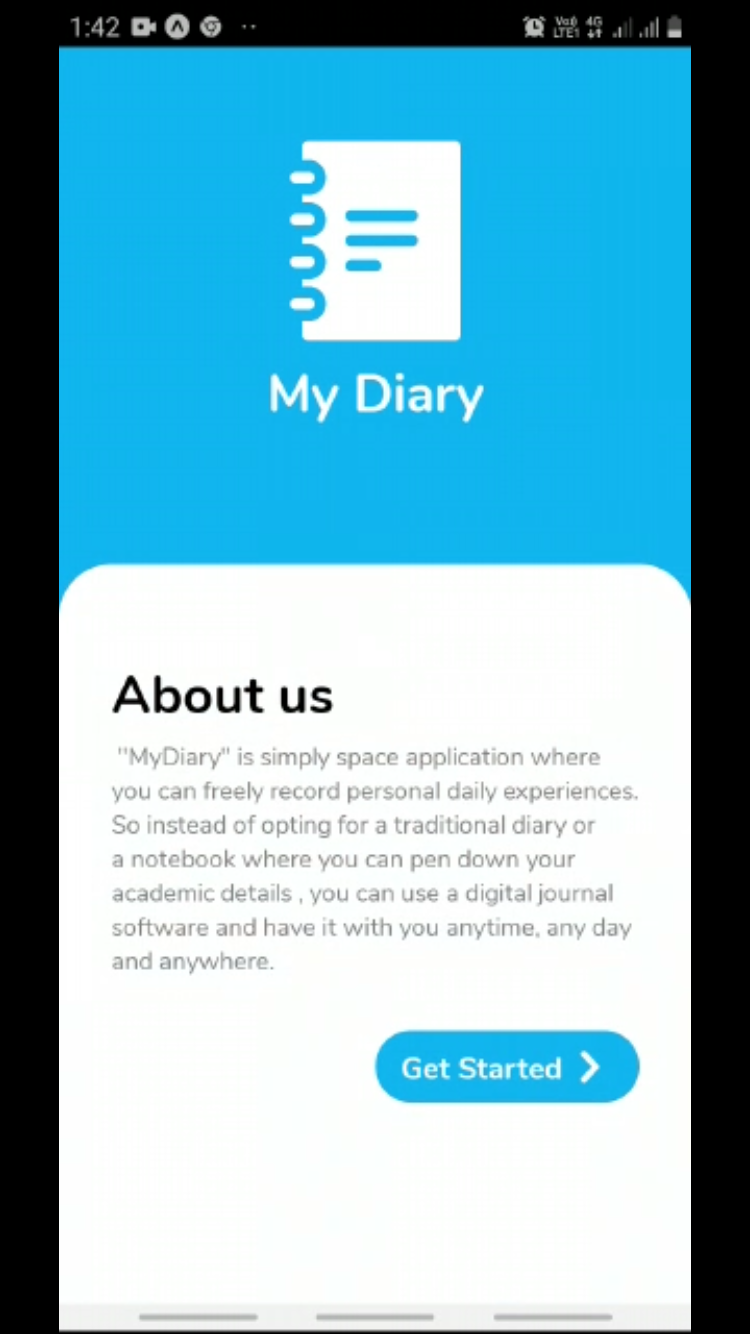
\includegraphics[width=0.49\textwidth]{register-aboutus.PNG}%
    }
\end{figure}
Here the user can register yourself by below feilds with the option sign up. After the sign up process the application will be displayed by the About us feild "description of application" and then you are logged in.


\begin{figure}[h]
\makebox[\textwidth]{%
    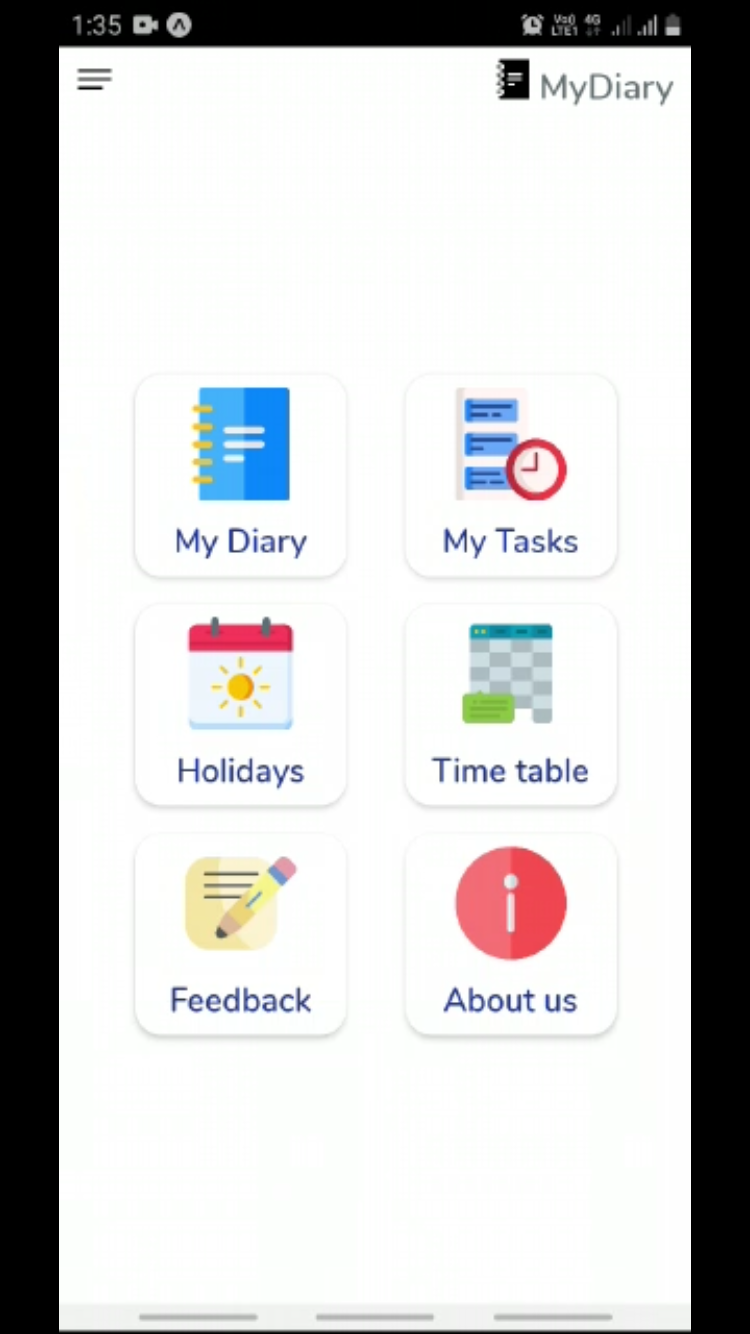
\includegraphics[width=0.59\textwidth]{home.PNG}%
     }
\end{figure}
After the login process, home page will be displayed with the different modules: "My Dairy","My Tasks","Holidays","Time Table","Feedback","About us".

\newpage
\begin{figure}[h]
\makebox[\textwidth]{%
    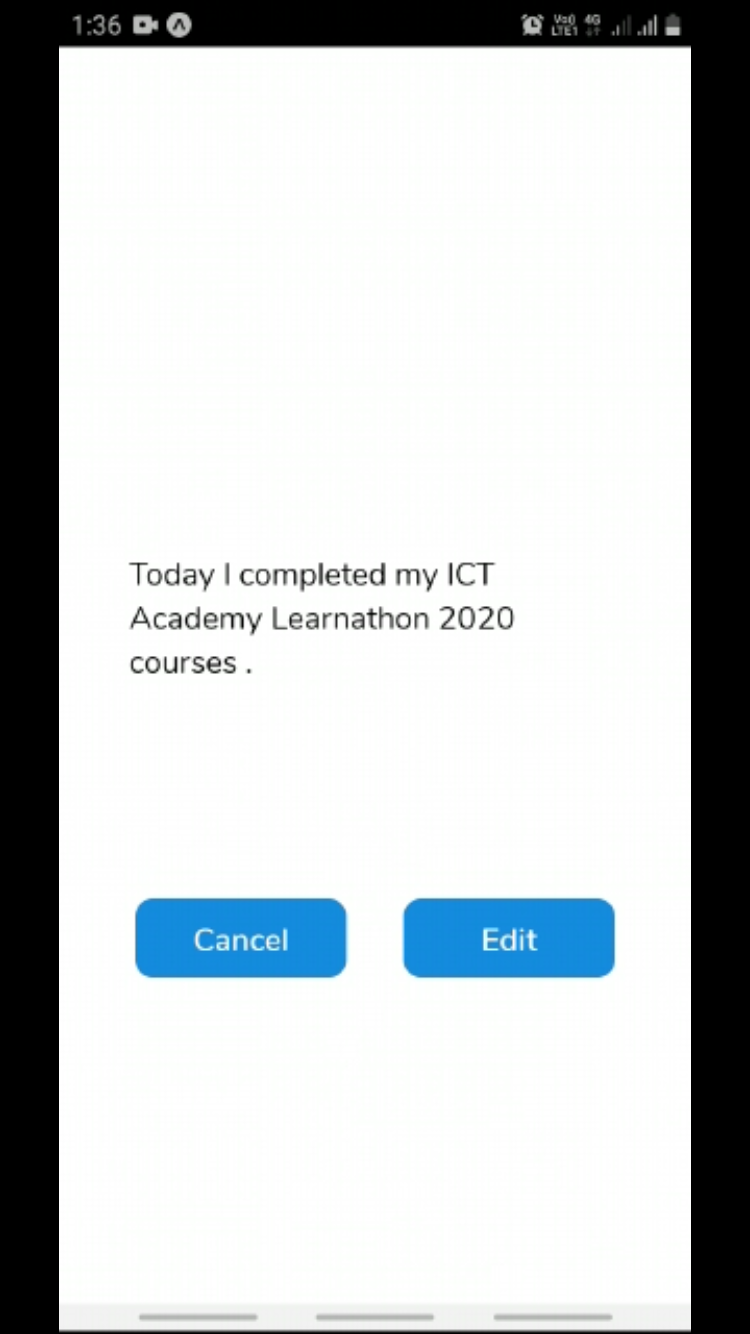
\includegraphics[width=0.59\textwidth]{mydaiy1.PNG}%
    \hfill
    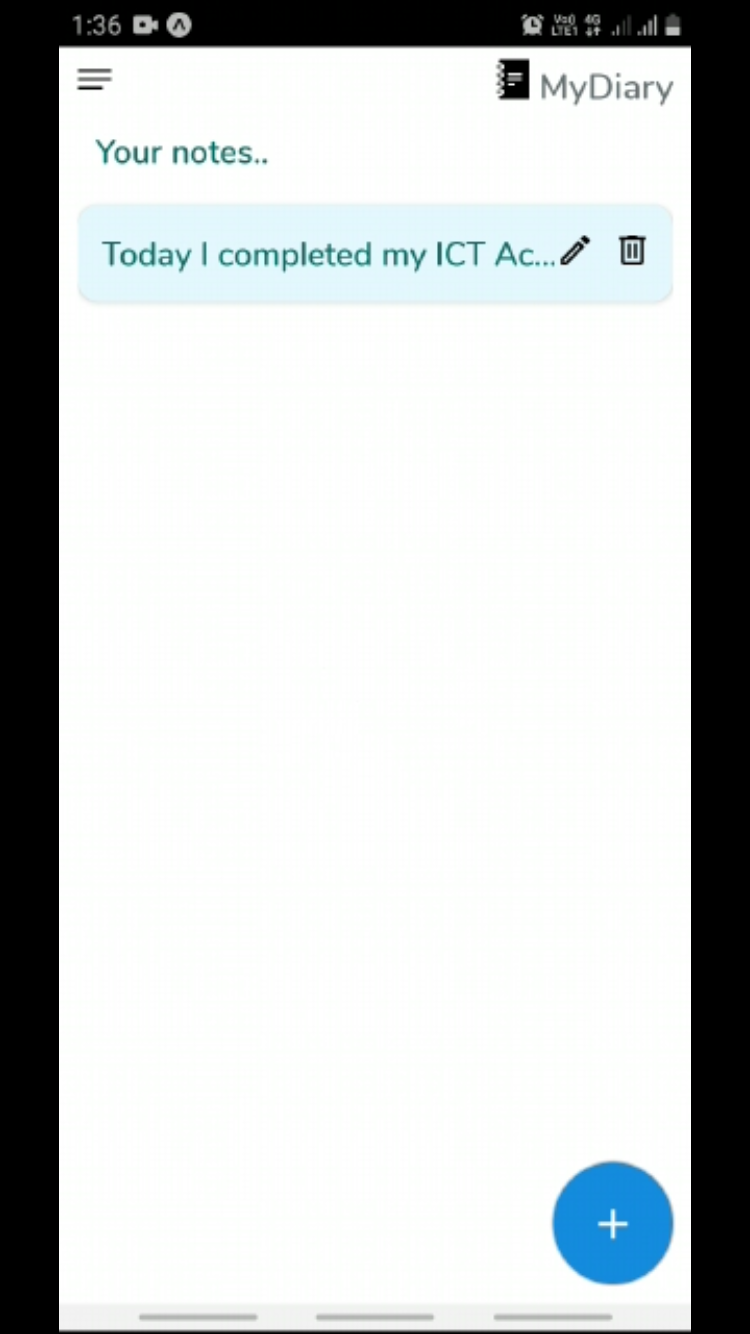
\includegraphics[width=0.59\textwidth]{mydaiy2.PNG}%
    }
\end{figure}
In the module "My Dairy", the user can write down daily notes as in their forms (personal,private) and can edit whenever they want.

\newpage
\begin{figure}[h]
\makebox[\textwidth]{%
    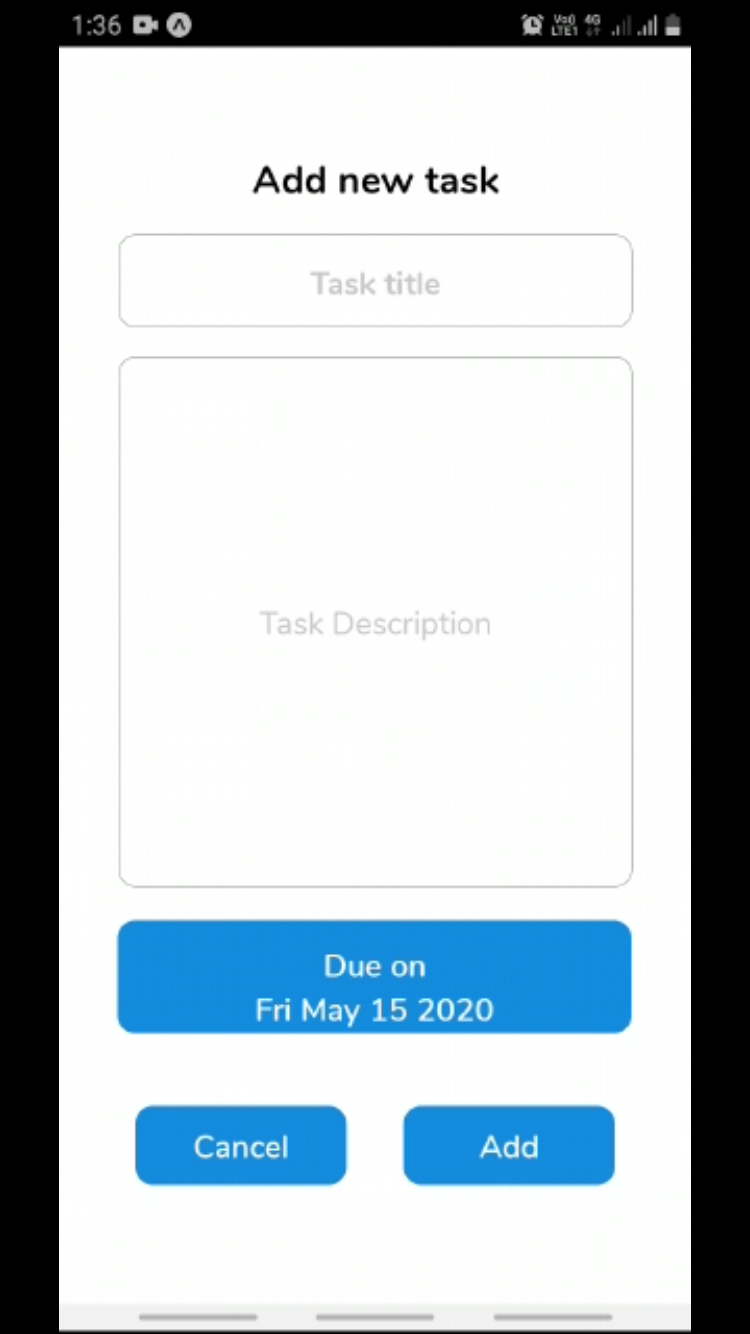
\includegraphics[width=0.32\textwidth]{task1.PNG}%
    \hfill    
    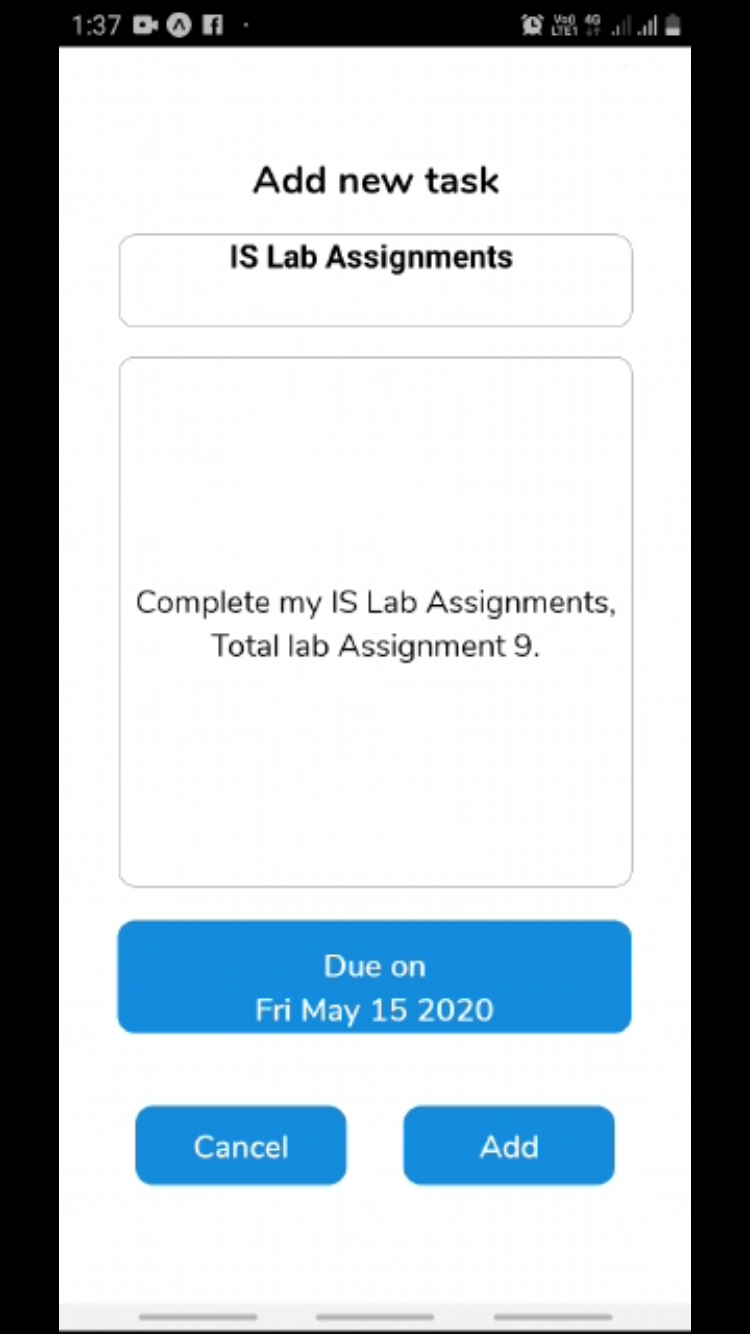
\includegraphics[width=0.32\textwidth]{task2.PNG}%
    \hfill
    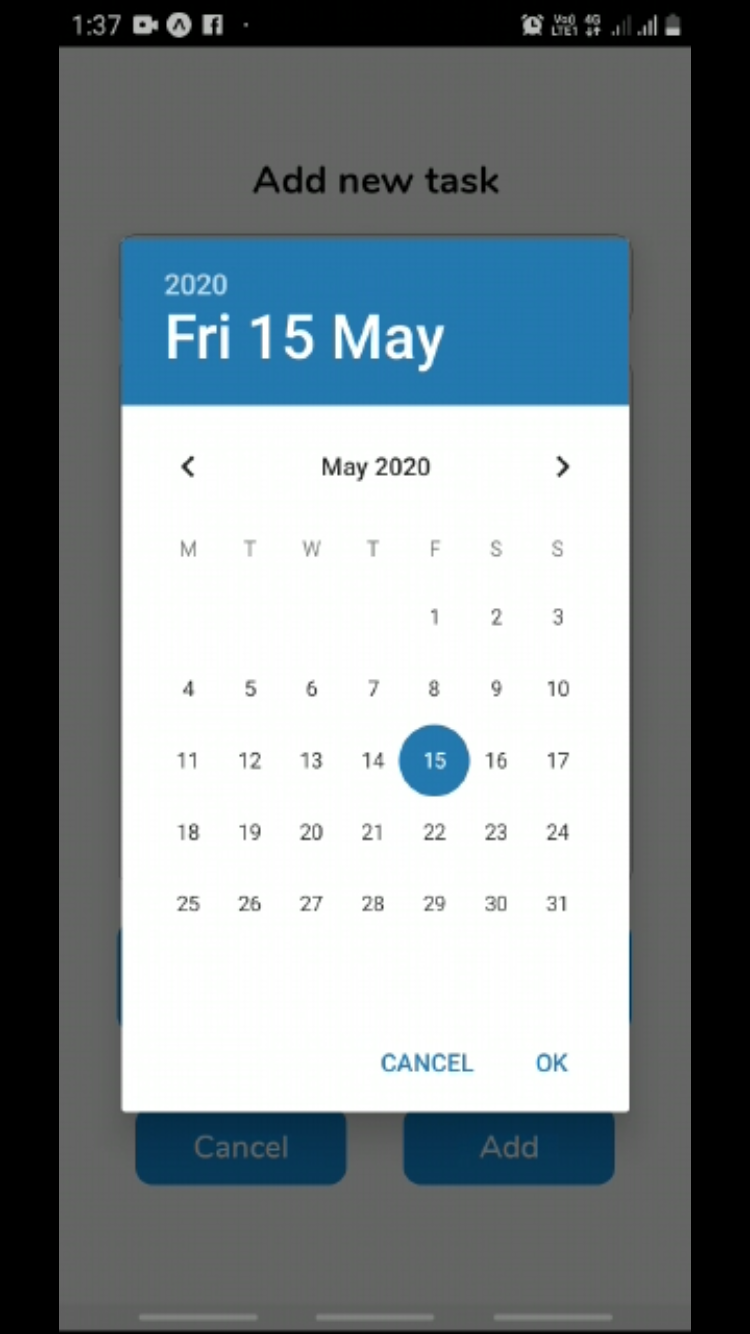
\includegraphics[width=0.32\textwidth]{task3.PNG}%
   }\\[0.5cm]%
   \makebox[\textwidth]{%
   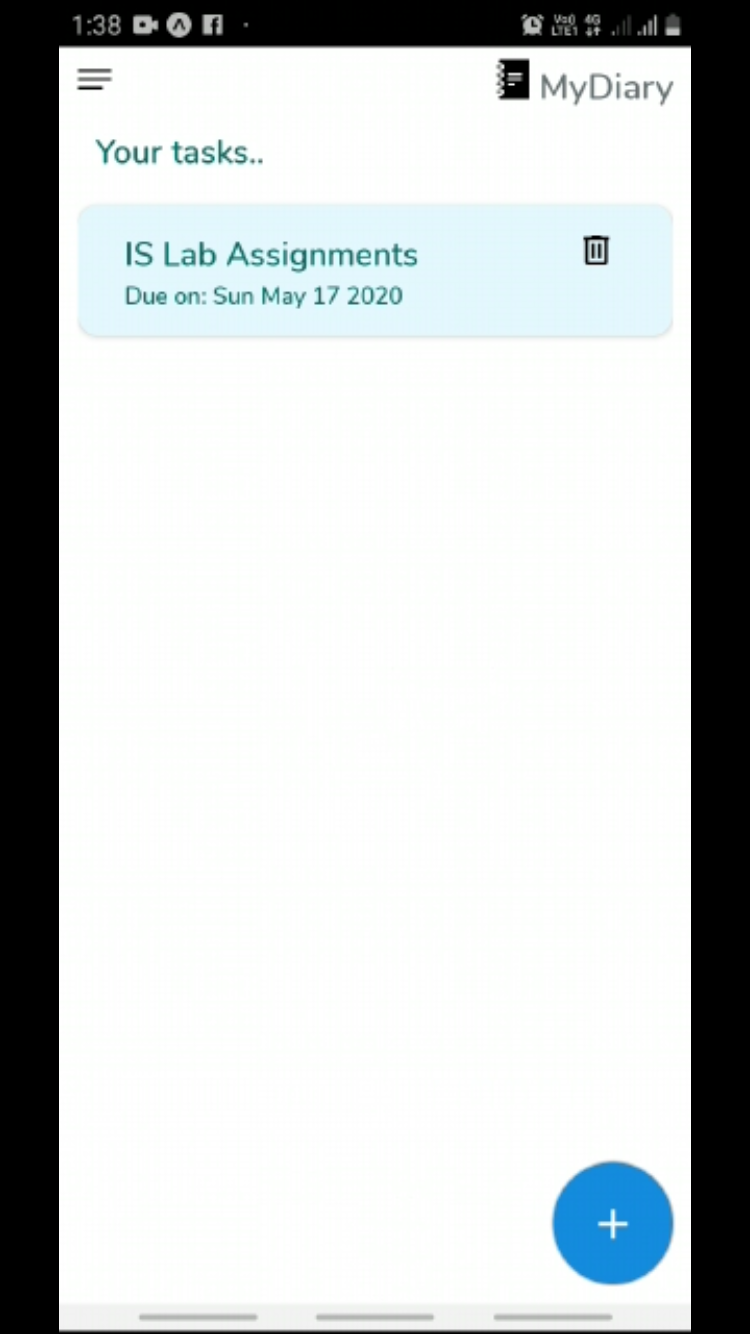
\includegraphics[width=0.32\textwidth]{task4.PNG}%
   \hfill
   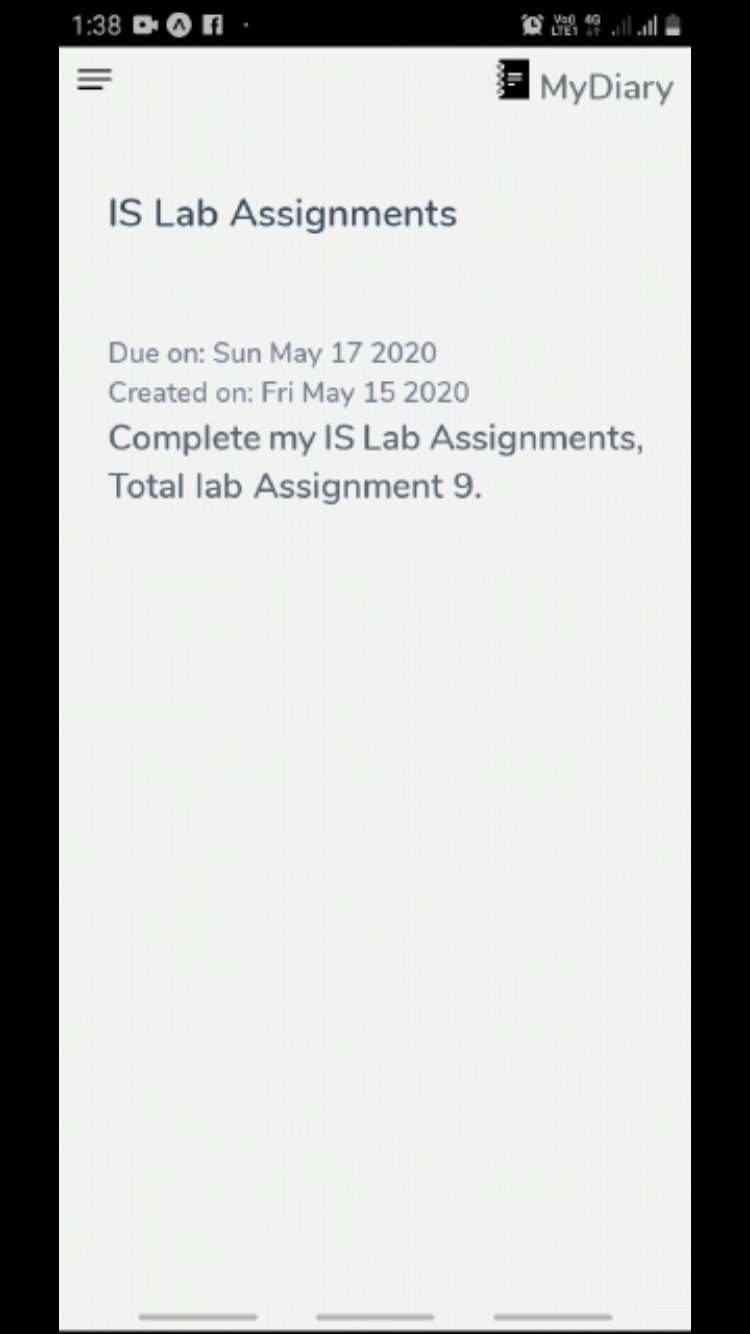
\includegraphics[width=0.32\textwidth]{task5.PNG}%
   }%
\end{figure}
In this module "My Tasks", the user can add title of their choice and with it they can add their task description in detail for better convenience. After the description, the user can allocate a date so that the application can make a notificationary remainder and the tasks will be displayed with their allocated dates.

\newpage
\begin{figure}[h]
\makebox[\textwidth]{%
    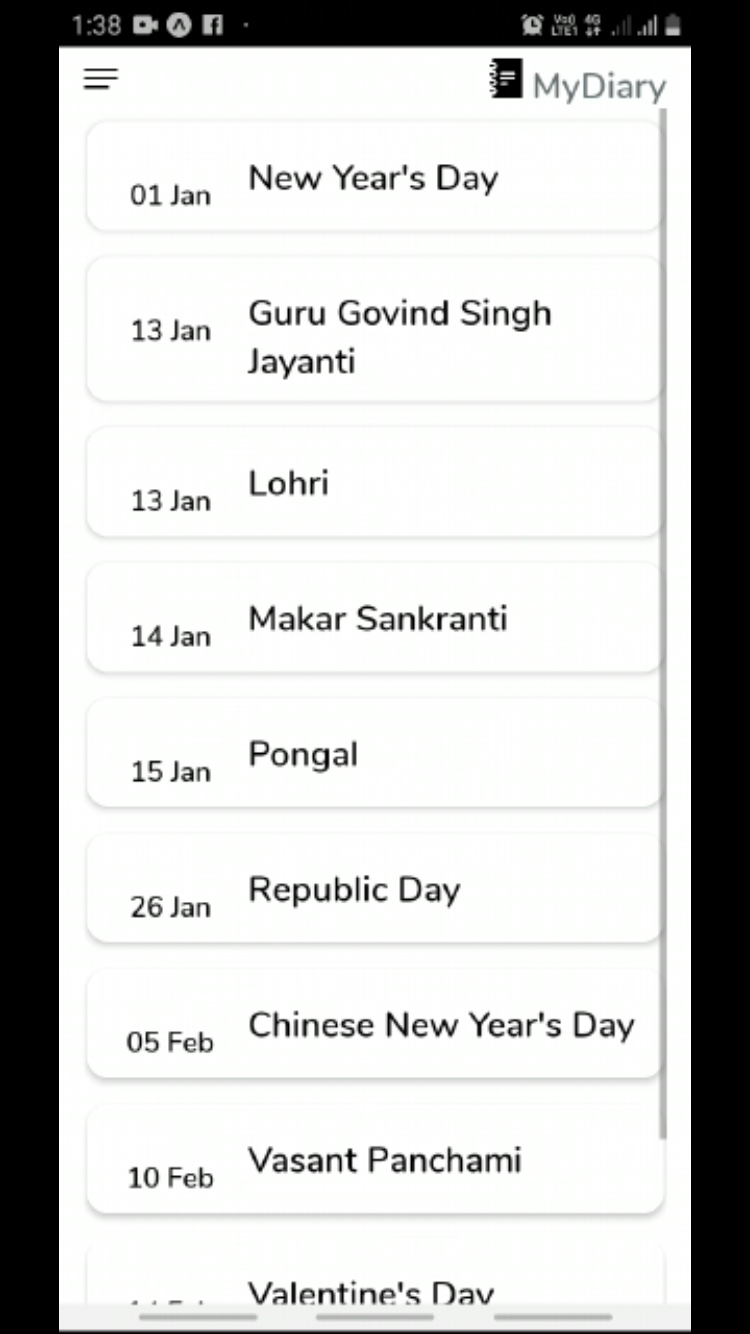
\includegraphics[width=0.59\textwidth]{holiday.PNG}%
     }
\end{figure}
The module "Holidays" will help the user to know about the holiday schedule as per the allocated dates.The user cannot have access to this module.

\newpage
\begin{figure}[h]
\makebox[\textwidth]{%
    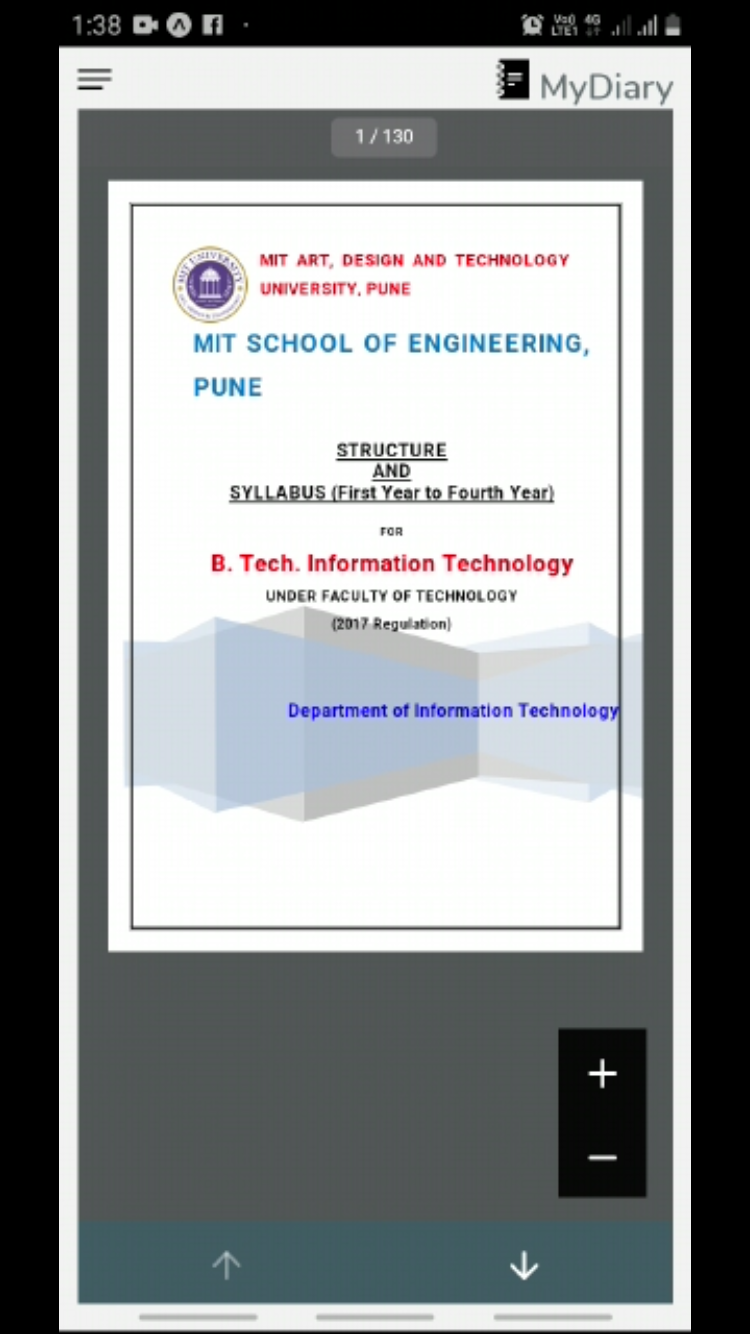
\includegraphics[width=0.59\textwidth]{timetable.PNG}%
     }
\end{figure}
"Time Table" module would display the timetable as per administrator allocation .The user cannot have access to this module.

\newpage
\begin{figure}[h]
\makebox[\textwidth]{%
    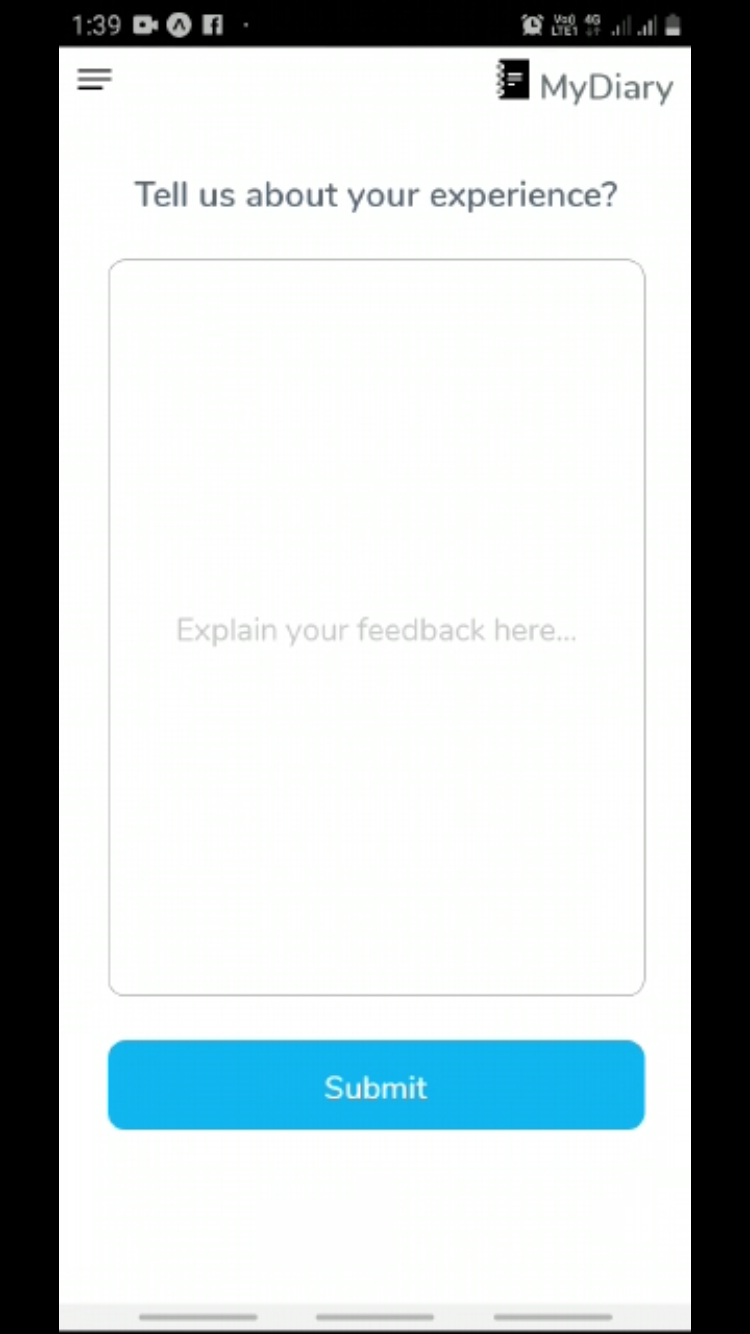
\includegraphics[width=0.32\textwidth]{feedback1.PNG}%
    \hfill    
    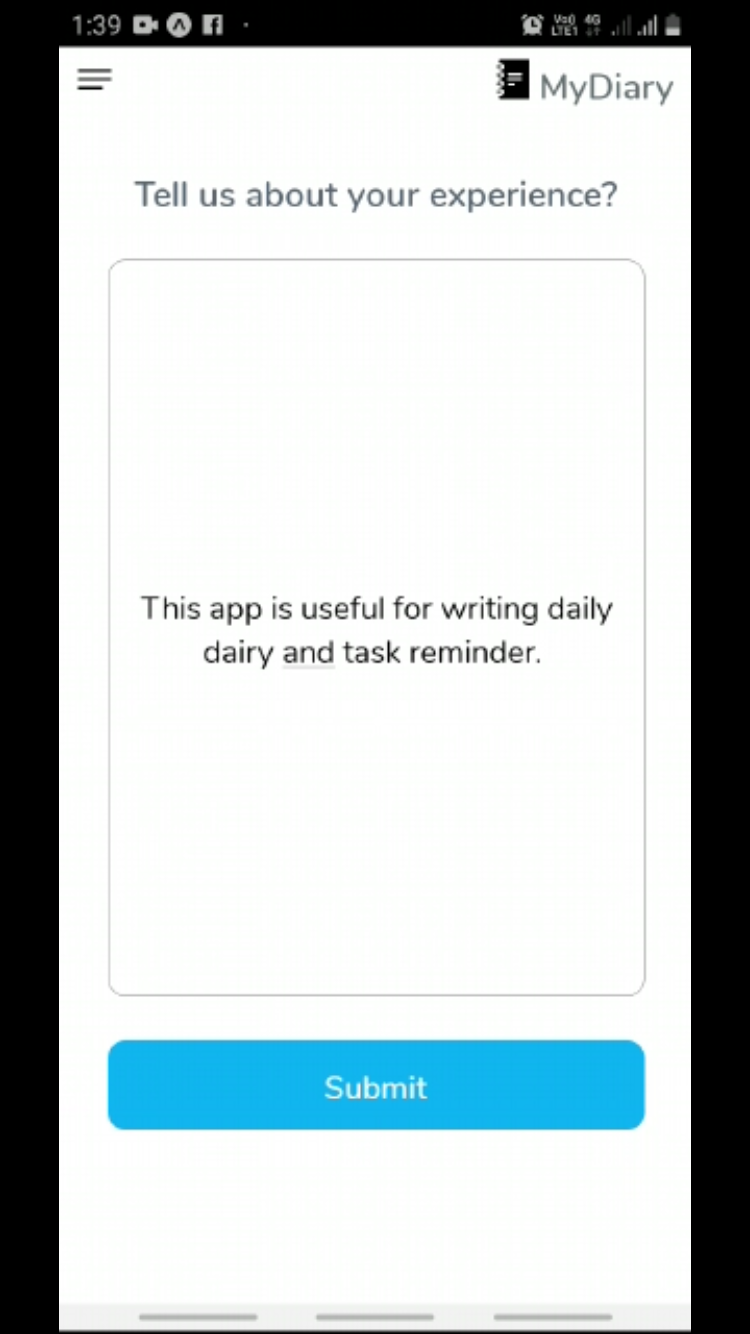
\includegraphics[width=0.32\textwidth]{feedback2.PNG}%
     }\\[0.5cm]%
   \makebox[\textwidth]{%
   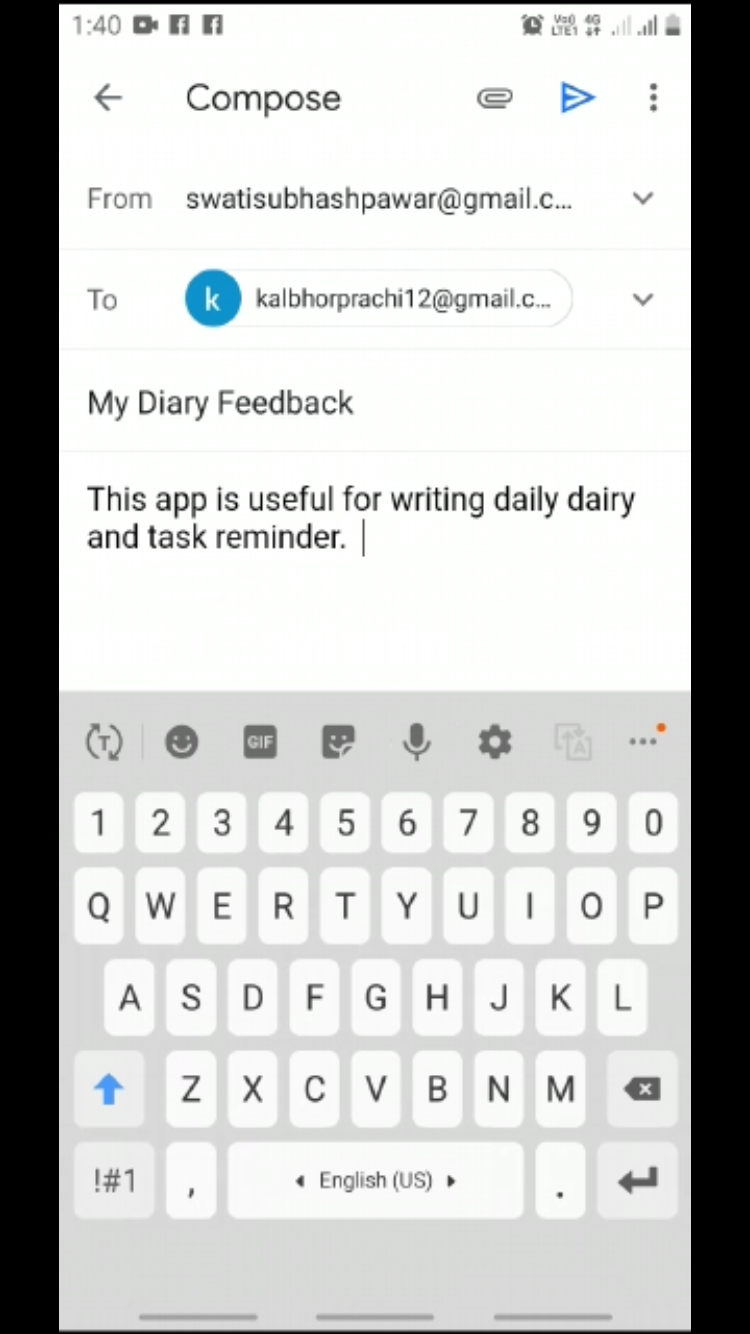
\includegraphics[width=0.32\textwidth]{feedback3.PNG}%
     }%
\end{figure}
The user can give their feedback about the application through "Feedback" module. It would direct be reported to the administrator's mail server.

\newpage
\begin{figure}[h]
\makebox[\textwidth]{%
    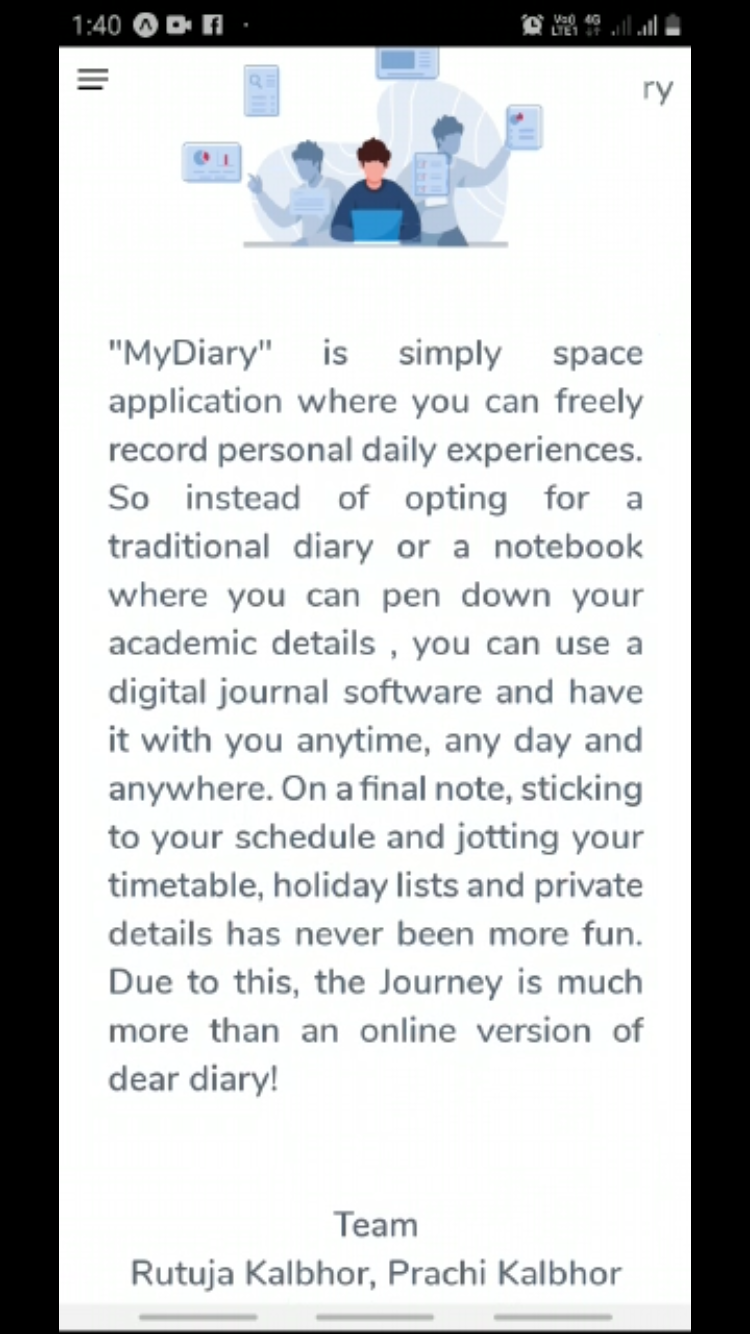
\includegraphics[width=0.59\textwidth]{aboutus.PNG}%
     }
\end{figure}
"About us" module displays the descriptive information about the application, so that the user can know about the convenient platform and to enhance the punctuality of the user.



\chapterfont{}
\setcounter{secnumdepth}{4}
\chapter {APPLICATIONS}
\section{Applications}
\Large
\begin{enumerate}[label=\roman*.]
\item Easy to understand and user friendly.
\item Secure application for students.
\item Person can update dairy anywhere anytime. 
\item User can have multiple dairy for multiple purpose.
\item Each dairy is secured with individual password.
\item Feature like feedback module.
\item Reminders, Notifications and Updates.
\item Special feature of Time Table notification module.
\end{enumerate}


\chapterfont{}
\setcounter{secnumdepth}{4}
\chapter {CONCLUSION AND FUTURE SCOPE}
\section{Conclusion and Future Scope:}
We have implemented the proposed application for writing diary in an interesting way and to change the conventional diary writing method. This project is intended to provide complete solutions for users who want to maintain records of their notes and add tasks as their remainders. In future, the foremost explore we want to do is add more security by adding authentication of OTP system. We would add notifications to the timetable module for keeping us updated on our upcoming lectures.This project helped us to enhance our skills in programming field of the software development. \\
\\
\\
\\
\\
\\
\\

The references for this report are \cite{sohn2008diary} , \cite{brown2000electronic} , \cite{adeyanjudevelopment} , \cite{lev2019viewing} and \cite{park2016digital}.

\bibliographystyle{ieeetr}
\bibliography{biblography} 




\end{document}
